\documentclass{article}%
\usepackage[T1]{fontenc}%
\usepackage[utf8]{inputenc}%
\usepackage{lmodern}%
\usepackage{textcomp}%
\usepackage{lastpage}%
\usepackage[tmargin=4cm,rmargin=2cm,lmargin=4cm,bmargin=3cm]{geometry}%
\usepackage[spanish]{babel}%
\usepackage[pages=all]{background}%
\backgroundsetup{placement=center,
 angle=0, scale=1, contents={
\includegraphics{Membrete.pdf}}, opacity=1}
%
\usepackage{ragged2e}%
\usepackage{xcolor}%
\usepackage{subcaption}%
\usepackage{graphicx}%
%
%
%
\begin{document}%
\normalsize%
\begin{center}%
\textcolor{white}{ 
HH
}%
\linebreak%
\linebreak%
\linebreak%
\linebreak%
\linebreak%
\linebreak%
\linebreak%
\linebreak%
\linebreak%
\linebreak%
\linebreak%
\linebreak%
\linebreak%
\linebreak%
\linebreak%
\begin{Huge}%
PROPUESTA DE VALOR PARA LA CONSTRUCCIÓN DE UNA HORNILLA%
\end{Huge}%
\linebreak%
\linebreak%
\linebreak%
\linebreak%
\linebreak%
\linebreak%
\linebreak%
\linebreak%
\linebreak%
\linebreak%
\begin{Large}%
Presentado por: AGROSAVIA%
\end{Large}%
\linebreak%
\begin{small}%
(Corporación Colombiana de Investigación Agropecuaria)%
\end{small}%
\end{center}%
\newpage%
\begin{large}%
 %
\textcolor{white}{ 
HH
}%
\linebreak%
Bogotá D.C., %
\ {\today}%
\newline%
 \newline%
%
\linebreak%
\newline%
Señor (es):%
\newline%
ss%
\newline%
Barbosa, Santander.%
\newline%
 \newline%
%
\newline%
Apreciado(s) productor(es):%
\newline%
 \newline%
%
Con base en la información suministrada, está aplicación propone (ver Sección 1) la construcción de una hornilla Plana de una camara con capacidad de 75 kg/h (la eficiencia estimada de la hornilla es del 41\%). ; adecuada para el procesamiento de hasta 1.125 ha de caña, con una producción de 54 t/mes y un periodo vegetativo de 16.0 meses. Teniendo en cuenta que se realizan 2 moliendas al mes se estableció una jornada laboral de 6 días a la semana de 12 horas laborables cada una.\newline%
 Además, la aplicación estima que para garantizar una operación apropiada de la hornilla  se requiere de un área disponible de al menos 322 m²%
, cuya productividad puede aumentar al incorporar el sistema de recuperación de calor (hasta 100 kg/h) como se muestra en las tablas del análisis financiero y al final del informe. No obstante, la corporación ofrece los siguientes servicios de asistencia técnica para ajustar los valores provistos en esta propuesta de valor:%
\begin{itemize}%
\item%
Estudio detallado para la construcción e instalación de la hornilla.%
\item%
Al menos tres visitas técnicas de dos funcionarios de AGROSAVIA para la puesta en marcha y capacitación de los operarios en el manejo de la hornilla y en la producción de panela saborizada, granulada o moldeada en presentación pastilla de chocolate.%
\item%
Entrega de un ejemplar de la guía tecnológica para el manejo integral del sistema productivo de la caña panelera y una para el mantenimiento de la hornilla.%
\end{itemize}%
Cualquier inquietud AGROSAVIA está presta a atenderla.\newline%
Cordial saludo.\newline%
\newline%
 \newline%
 \newline%
AGROSAVIA (Corporación colombiana de investigación agropecuaria)%
\newline%
 \newline%
 Nota: Está propuesta de valor se basa en condiciones del terreno ideales y estacionarias, por lo que, AGROSAVIA no se hace responsable de la reproducción total o parcial del material aquí suministrado sin una aprobación corporativa.%
\end{large}%
\newpage%
\begin{large}%
 %
\begin{Large}%
\textbf{Contenido}%
\end{Large}%
\begin{itemize}%
\item%
Sección 1%
\begin{itemize}%
\item%
Información del usuario.%
\item%
Características de la caña sembrada.%
\item%
Características del molino.%
\item%
Consideraciones generales para el manejo de la hornilla.%
\item%
Análisis financiero.%
\end{itemize}%
\item%
Sección 2%
\begin{itemize}%
\item%
Diagramas mecánicos de la hornilla.%
\item%
Diagramas mecánicos de la camára.%
\item%
Diagramas mecánicos de la chimenea.%
\item%
Diagramas mecánicos del ducto.%
\item%
Diagramas mecánicos de la hornilla con recuperador de calor.%
\end{itemize}%
\end{itemize}%
\end{large}%
\newpage%
\begin{center}%
\textcolor{white}{ 
HH
}%
\linebreak%
\linebreak%
\linebreak%
\linebreak%
\linebreak%
\linebreak%
\linebreak%
\linebreak%
\linebreak%
\linebreak%
\linebreak%
\linebreak%
\linebreak%
\linebreak%
\linebreak%
\begin{Huge}%
SECCIÓN 1:%
\end{Huge}%
\linebreak%
\begin{Huge}%
INFORMACIÓN TÉCNICA Y FINANCIERA%
\end{Huge}%
\end{center}%
\newpage%
\begin{center}%
\begin{Huge}%
DATOS DEL USUARIO%
\end{Huge}%
\linebreak%
\end{center}%
\begin{tabular}{lccccl}%
\textbf{Nombre de usuario}& & & & &ss\\%
\textbf{Correo}& & & & &ss@sss\\%
\textbf{Telefono}& & & & &123456\\%
\textbf{Pais}& & & & &Colombia\\%
\textbf{Departamento}& & & & &Santander\\%
\textbf{Ciudad}& & & & &Barbosa\\%
\textbf{Área caña sembrada}& & & & &18 ha\\%
\textbf{Área proyectada para cultivo en los proximos 5 años}& & & & &0\\%
\textbf{Número de moliendas al mes}& & & & &2\\%
\textbf{Días de trabajo de la hornilla a la semana}& & & & &6\\%
\textbf{Horas de trabajo de la hornilla al día}& & & & &12\\%
\textbf{Variedades de caña sembrada}& & & & &1\\%
\textbf{Altura media sobre el nivel del mar}& & & & &1300 m\\%
\textbf{Nivel freático}& & & & &desde 100 m\\%
\textbf{Caña producida por hectárea (t/ha)}& & & & &48.375\\%
\textbf{Periodo vegetativo}& & & & &16.0 mes(es)\\%
\end{tabular}%
\newpage%
\begin{center}%
\begin{Huge}%
CARACTERÍSTICAS DE LAS VARIEDADES DE CAÑA SELECCIONADAS%
\end{Huge}%
\linebreak%
\end{center}%
\begin{tabular}{lcccccl}%
\textbf{Variedad de Caña 1}& & & & & &RD75{-}11\\%
\textbf{Grados Brix de la caña 1}& & & & & &19.2\\%
\textbf{pH}& & & & & &5.7\\%
\textbf{Azúcares reductores (\%)}& & & & & &0.9\\%
\textbf{Sacarosa (\%)}& & & & & &18.2\\%
\textbf{Pureza (\%)}& & & & & &94.8\\%
\textbf{Fósforo (ppm)}& & & & & &66\\%
\textbf{>{-}{-}{-}{-}{-}{-}{-}{-}{-}{-}{-}{-}{-}{-}{-}{-}{-}{-}{-}{-}{-}{-}{-}{-}{-}{-}{-}{-}{-}{-}{-}{-}{-}<}& & & & & &>{-}{-}{-}{-}{-}{-}{-}{-}{-}{-}{-}{-}{-}{-}{-}{-}{-}{-}{-}{-}{-}{-}{-}{-}{-}{-}{-}{-}{-}{-}{-}{-}{-}<\\%
\end{tabular}%
\linebreak%
\newline%
%
\linebreak%


\begin{figure}[h!]%
\begin{subfigure}{0.33\linewidth}%
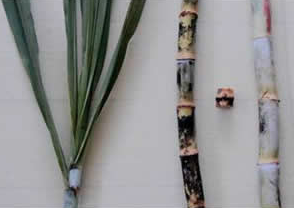
\includegraphics[width=0.95\linewidth]{Cana/RD75-11.png}%
\caption{Variedad de caña 1}%
\end{subfigure}%
\linebreak%
\newpage%
\end{figure}

%
\newpage%
\textcolor{white}{ 
HH
}%
\newpage%
\begin{center}%
\begin{Huge}%
MOLINOS PRESELECCIONADOS PARA ESTE DISEÑO%
\end{Huge}%
\linebreak%
\end{center}%
\begin{tabular}{lcccccl}%
\textcolor{red}{ 
\textbf{VALOR APROXIMADO DE UN MOLINO: }
}& & & & & &\textcolor{red}{ 
\$ 9,150,000.00
}\\%
\end{tabular}%
\linebreak%
\begin{tabular}{ccccc}%
MARCA&MODELO&KG POR HORA&DIESEL O GASOLINA (HP)&ELÉCTRICO (HP)\\%
&&&&\\%
MIRACLE&MRC{-}EB05&500&4&3\\%
Panelero&R2{-}S&500&10&5\\%
\linebreak%
\newline%
%
\linebreak%
\end{tabular}%


\begin{figure}[h!]%
\begin{subfigure}{0.33\linewidth}%
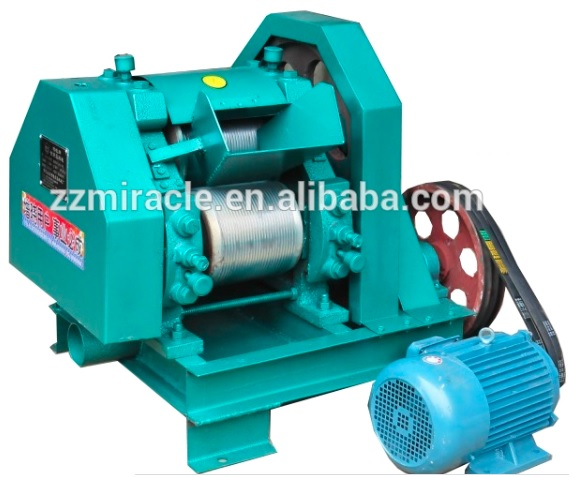
\includegraphics[width=0.95\linewidth]{Molinos/MRC-EB05.jpg}%
\caption{MRC{-}EB05}%
\end{subfigure}%
\begin{subfigure}{0.33\linewidth}%
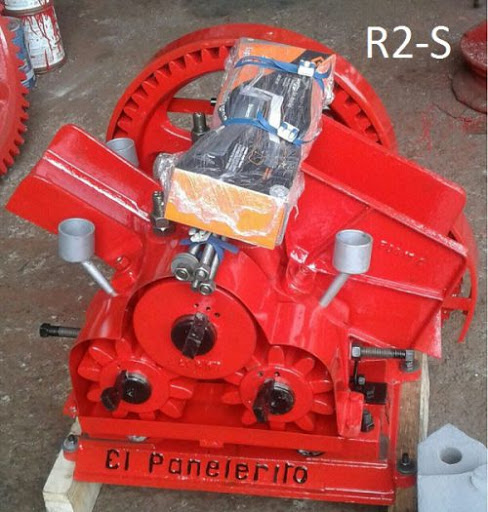
\includegraphics[width=0.95\linewidth]{Molinos/R2-S.jpg}%
\caption{R2{-}S}%
\end{subfigure}%
\linebreak%
\newpage%
\end{figure}

%
\newpage%
\textcolor{white}{ 
HH
}%
\newpage%
\begin{large}%
 %
\begin{Large}%
\textbf{Consideraciones para el manejo de la hornilla}%
\end{Large}%
\newline%
 \newline%
El trapiche panelero es un lugar donde se procesa la caña de azúcar para producir la panela. Está constituido por las áreas de molienda, prelimpieza, hornilla, moldeo y almacenamiento.%
\newline%
 La hornilla panelera, está conformada, por el cenicero, la cámara, la chimenea y el ducto, sobre el cual se asientan directamente los intercambiadores de calor, en los que se deposita el jugo. En la hornilla panelera, se genera y transfiere el calor necesario para concentrar en un sistema de evaporación abierta, el jugo de la caña; de tal forma que la cantidad de energía aprovechada se relaciona directamente con el suministro de aire y bagazo, la eficiencia de la combustión, y la cantidad de energía disipada a los alrededores. Estas variables de operación y transferencia se relacionan entre si y debido a su complejidad y cantidad, dificultan las tareas de manipulación y diseño de la hornilla.%
\begin{Large}%
\textbf{\newline%
 \newline%
 Manejo de las hornillas paneleras}%
\end{Large}%
\begin{itemize}%
\item%
Tenga en cuenta las siguientes indicaciones.%
\begin{itemize}%
\item%
Durante las pruebas iniciales y periodos de capacitación, los operarios que manejan la hornilla deben tener experiencia para evitar la disminución en la calidad de la panela y vida util de los equipos instalados.%
\item%
El trabajo continuo de la hornilla aumenta la capacidad de producción y evita la perdida de energía, puesto que, al no enfriarse durante las horas de la noche se reduce el efecto del cambio térmico sobre los ladrillos de la estructura.%
\item%
La combustión en la hornilla será buena, si se alimenta con pequeñas cantidades de bagazo cada 150 segundos y la válvula de la chimenea tiene una apertura 60° para garantizar un flujo de aire suficientemente alto que produzca llama, sin arrastrar combustible en los gases residuales.%
\item%
La entrada de aire por orificios diferentes a los proyectados en el diseño inicial debe evitarse a toda costa, para aumentar la eficiencia de la combustión y reducir el material particulado de los gases en la chimenea.%
\item%
Elimine obstáculos en las entradas de aire diseñadas para la hornilla y retire periódicamente la ceniza la parrilla para evitar la formación de escoria.%
\item%
El cenicero y su entrada deben mantenerse despejada a fin de no obstruir el paso del aire.%
\item%
El bagazo para alimentar la hornilla debe tener las condiciones de humedad mencionadas en el diseño.%
\item%
Almacene el bagazo por dos semanas en la bagacera, y así, obtendrá un bagazo con al menos un 30\% de humedad.%
\item%
Ajuste el tiro de la chimenea usando la válvula mariposa cuando tenga bagazo con mayor humedad.%
\item%
La válvula no opera en tiempo real y cuando se encuentra a medio cerrar se aumenta la velocidad de calentamiento en la zona de evaporación al pie de la entrada del bagazo. Sin embargo, cuando se encuentra abierta el calentamiento se presenta al pie de la chimenea.%
\item%
El tiempo de residencia del jugo en la hornilla, influye en la calidad de la panela y este es directamente proporcional al aumento de los azucares invertidos.%
\item%
Las falcas en las pailas son de seguridad, no deben usarse para contener una mayor cantidad de jugo. Por tanto para aumentar la transferencia de calor al jugo y mejorar la calidad de la panela es importante manejar la cantidad de jugo mínima en cada paila.%
\item%
El nivel del jugo en las pailas semiesféricas, siempre debe estar por encima de la línea de contacto de los gases de combustión con la paila a fin de evitar quemadura en la panela.%
\item%
La paila clarificadora debe calentar lo más rápido posible para que permita remover la cachaza. Además, la velocidad mínima de calentamiento debe ser de 1.5°C/min.%
\item%
Elimine residuos de la caña o jugos presentes sobre la superficie de las pailas concentradoras de panela y cachaza periódicamente, para que el producto se pegue al fondo. Lo cual disminuye el paso del calor y deterioran la calidad del producto.%
\end{itemize}%
\end{itemize}%
\begin{Large}%
\textbf{Mantenimiento de la hornilla}%
\end{Large}%
\begin{itemize}%
\item%
Después de cada molienda.%
\begin{itemize}%
\item%
Limpie y desinfecte las instalaciones, pailas, equipos y utensilios, antes de iniciar nuevamente la producción de panela.%
\item%
Un encelamiento de los moldes, utensilios de madera y prelimpiadores.%
\item%
Dejar en remojo con agua limpia las pailas durante el enfriamiento de la hornilla.%
\item%
Retirar la ceniza del cenicero y el ducto.%
\end{itemize}%
\end{itemize}%
\begin{itemize}%
\item%
Cada seis moliendas.%
\begin{itemize}%
\item%
Retirar el hollín formado en la superficie de las pailas, por donde se transfiere el calor.%
\item%
Limpiar los ductos de las pailas piro{-}tubulares, con ayuda de un raspador o un costal de fique.%
\end{itemize}%
\end{itemize}%
\begin{itemize}%
\item%
Cada seis meses.%
\begin{itemize}%
\item%
Realice una limpieza general e inspección del estado de los ductos.%
\item%
Realice un mantenimiento de las paredes del ducto y la cámara.%
\end{itemize}%
\end{itemize}%
\begin{Large}%
\textbf{Recomendaciones de construcción del trapiche}%
\end{Large}%
\begin{itemize}%
\item%
Algunos parámetros para tener en cuenta son.%
\begin{itemize}%
\item%
El suministro de agua ser potable y continuo.%
\item%
Los alrededores de las fábricas deben estar libre de posibles focos de infección.%
\item%
Las áreas de trabajo de cada subproceso deben estar delimitadas.%
\item%
Las áreas de procesamiento y empaque deben estar separadas de las áreas de recepción y desechos.%
\item%
Las uniones de las baldosas deben recubrirse de materiales plásticos que faciliten la limpieza.%
\item%
Las salientes de las paredes, dinteles de ventanas y suspensiones del techo deben ser curvas e inclinadas.%
\item%
Los pisos y las paredes se deben construir con materiales anticorrosivos, no absorbentes y de alto transito.%
\item%
Las áreas de procesos deben tener en el centro un canal de drenaje con 3° de inclinación y una parrilla removible para realizar su limpieza.%
\item%
Los pisos deben tener una leve inclinación (3°) para realizar el drenado.%
\item%
Los desagües deben tener rejillas de seguridad para impedir el paso de animales.%
\item%
Los ambientes debe ser ventilados.%
\item%
Los vapores deben contar con su propio escape para evitar la presencia de moho en paredes y techos.%
\item%
Los ductos de ventilación deben estar cubiertos de mallas protectoras.%
\item%
Los ambientes deben estar bien iluminados.%
\item%
Las bases o cimientos deben ser lisos para evitar la presencia de insectos o residuos.%
\item%
Los espacios entre los equipos o equipos y paredes deben estar sellados.%
\item%
Los baños, habitaciones y casilleros, deben estar aseados y alejados de las áreas de procesamiento y producto terminado.%
\item%
Las diferentes áreas deben disponer de un sitio para el aseo de las manos con sus respectivos implementos, tales como; jabón líquido, cepillos y toallas desechables.%
\end{itemize}%
\end{itemize}%
\begin{Large}%
\textbf{Higiene y desinfección en el trapiche}%
\end{Large}%
\begin{itemize}%
\item%
Tenga en cuenta las siguientes indicaciones para su cuidado personal.%
\begin{itemize}%
\item%
El objetivo de la higiene en los alimentos es alargar la vida útil del producto, y proteger al consumidor final de las enfermedades producidas al ingerir alimentos contaminados.%
\item%
La higienización de un trapiche requiere de una limpieza con detergente y de una esterilización industrial o satanización (desinfectante y bactericida).%
\item%
Los equipos y utensilios deben limpiarse y desinfectarse al final e inicio de cada molienda.%
\item%
La limpieza se realiza siguiendo estas pautas: proteger las materias prima y los productos terminados, raspar los residuos sólidos con una espátula sobre un recogedor y lavar con agua limpia, cepillo y detergente%
\item%
La esterilización se realiza con calor (vapor de agua, agua hirviendo), o un esterilizante químico (bactericida, desinfectante).Cuando se emplea agua caliente debe estar hirviendo (90°C) o en el caso del esterilizante químico puede usarse una solución clorada, de vinagre y una lechada de cal.%
\item%
Las soluciones desinfectantes deben aplicarse en solución con un rociador, empezando por la parte inferior.%
\item%
Antes de la esterilización la superficie debe estar limpia y totalmente escurrida.%
\item%
Las superficies en contacto con el alimento deben ser lisas, exentas de huecos, grietas y evitar las esquinas cuadradas.%
\item%
La industria de alimentos usa ampliamente el acero inoxidable y plásticos como el teflón por la facilidad de higienización, y su poca alteración al contacto con los alimentos.%
\item%
No debe usarse el cobre, bronce, estaño, aluminio, madera y zinc para las superficies que están en contacto con el alimento.%
\item%
No emplee en la limpieza esponjas o cepillos metálicos que rayen las superficies.%
\item%
Las pailas se lavan con arena de peña y esponja para desmancharla.%
\item%
Ningún tipo de rosca debe estar en contacto con el alimento.%
\item%
Se debe mantener una inclinación de superficies y tubería para el drenaje de 1 centímetro por metro.%
\item%
Se deben usar conexiones hidraulicas y uniones que sean de fácil limpieza.%
\item%
Se debe evitar la unión de acero inoxidable con otros metales.%
\item%
El hipoclorito ejerce una rápida acción bactericida sin dejar residuos tóxicos.%
\item%
No es aconsejable el uso de cloro en material de acero inoxidable.%
\item%
En la esterilización del acero inoxidable, puede utilizarse agua caliente, vapor o solución de 0.25 litros de vinagre en 10 litros de agua.%
\item%
Los materiales plásticos se deben lavar con una solución de 5.0 gramos de bicarbonato (2 cucharadas) en l0 litros de agua clorada y dejar secar durante 30 minutos.%
\item%
La esterilización del acero inoxidable puede hacerse con agua caliente, vapor o solución de 0.25 litros de vinagre en 10 litros de agua.%
\item%
Las superficies de madera se limpian con espátula para eliminar los residuos sólidos. Después remojar en detergente durante 5 minutos, luego cepillar, lavar con agua limpia, y finalmente rociar con solución de 12 gramos de cal (una cucharadita) en 10 litros de agua dejar secar.%
\item%
Los utensilios de madera se dejan en un recipiente plástico limpio, con solución de 12 gramos de cal (una cucharadita) en 10 litros de agua.%
\item%
Cambiar la solución donde se sumergen los utensilios de madera cada cuatro horas.%
\item%
Los utensilios y gaveras no deben dejarse sobre el suelo o superficies no desinfectadas.%
\item%
Evitar la caída de grasa mecánica en los alimentos.%
\end{itemize}%
\end{itemize}%
\end{large}%
\newpage%
\end{document}